\documentclass[11pt,twoside,a4paper]{article}
\usepackage[italian]{babel}
\usepackage{listings}
\usepackage{color}
\usepackage{mathtools}
\usepackage{biblatex}
\usepackage{subcaption}
%useful colors
\definecolor{mygreen}{rgb}{0,0.6,0}
\definecolor{mygray}{rgb}{0.5,0.5,0.5}
\definecolor{mymauve}{rgb}{0.58,0,0.82}
\definecolor{gray}{rgb}{0.4,0.4,0.4}
\definecolor{darkblue}{rgb}{0.0,0.0,0.6}
\definecolor{cyan}{rgb}{0.0,0.6,0.6}
%defining styles for listings
%java listings
\lstdefinestyle{octave}{
	basicstyle=\footnotesize,
	breakatwhitespace=false,
	breaklines=true,
	captionpos=b,
	commentstyle=\color{mygreen},
	frame=single,
	keywordstyle=\color{blue},
	language=octave,
	numbers=left,
	numbersep=5pt,
	numberstyle=\tiny\color{mygray},
	rulecolor=\color{black},
	showstringspaces=false,
	stepnumber=1,
	stringstyle=\color{mymauve},
	tabsize=2,
	title=\lstname
}
\begin{document}
\title{Classification on Pedobarography images}
\author{Luigi Lomasto, Marco Mecchia} 
\maketitle
\section{Introduzione al problema}
IL termine Pedobarography deriva dal latino \emph{pedes}, piede, e dal greco \emph{baros}, peso o pressione, e si riferisce allo studio dei campi di pressione della superficie plantare del piede su una superficie di supporto. La Pedobarography \'e spesso usata per l'analisi biomeccanica del movimento animale e per l'analisi della postura. In questo lavoro, il nostro obiettivo \'e quello di addestrare un sistema di Machine Learning in grado di classificare le immagini derivate dall'analisi statica, tramite Pattern Recognition Statistico.
Il resto del lavoro \'e organizzato come segue: nella sezione \ref{sec:dataset} viene descritto il dataset utilizzato nel lavoro, e il lavoro di preprocessing effettuato su di esso. Nella sezione \ref{sec:features} vengono descritte le feature scelte per addestrare il classificatore, e la loro convalida tramite metodi noti in letteratura. Nella sezione \ref{sec:classification} vengono descritti i classificatori utilizzati. Nella sezione \ref{sec:results} vengono illustrati i risultati, ed infine nella sezione \ref{sec:conclusions} vengono tratte le considirezioni su quanto fatto, ed analizzati alcuni possibili sviluppi futuri.

\section{Dataset ed obiettivi della classificazione}
\label{sec:dataset}
Il dataset utilizzato consiste in 100 immagini derivate dall'analisi statica di 100 pazienti diversi, ed \'e stato fornito dal dott. NOME DOTTORE in forma anonima. Un esempio di immagine \'e fornito in figura \ref{fig:immagineEsempio}. 
\begin{figure}
\centering
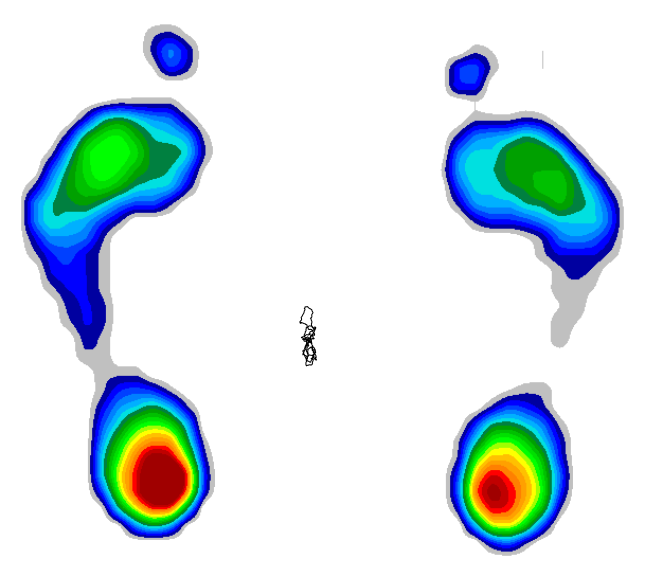
\includegraphics[height=100px, keepaspectratio]{4.png}
\label{fig:immagineEsempio}
\caption{Un immagine del dataset}
\end{figure}
Per ogni immagine ci \'e stata fornita anche la patologia di cui era affetto il piede del paziente, esse sono:
\begin{description}
\item[Piede Valgo] Sinistro, Destro, o Bilaterale.
\item[Piede Cavo] Sinistro, Destro, o Bilaterale.
\item[Piede Piatto] Sinistro, Destro, o Bilaterale.
\item[Piede Normale] Sinistro, Destro, o Bilaterale.
\end{description}

Tutte queste patologie non sono necessariamente esclusive: in particolare, un piede valgo pu\'o anche essere piatto o cavo. Per questo motivo, e per non gestire troppe classi di output, la classificazione \'e stata organizzata in maniera gerarchica, come si pu\'o vedere in figura \ref{fig:classificazioneGerarchica}.

FIGURA/DIAGRAMMA DI FLUSSO

Ogni immagine viene suddivisa in piede sinistro e piede destro. Sul piede singolo prima viene effettuata la classificazione cavo vs piatto, in quanto le classi sono mutualmente esclusive, dopodich\'e viene effettuata la classificazione valgo vs non valgo. Le informazioni sui piedi vengono combinate alla fine per stabilire se la patologia \'e bilaterale o meno.

\section{Preprocessing}
\label{sec:preprocessing}
Prima di estrarre le features, \'e stato necessario effettuare delle operazioni preliminari di pulizia e di normalizzazioni sulle immagini. In questa sezione vengono illustrate tutte le operazioni effettuate sulle immagine, fornendo le motivazioni che hanno portato ad ogni operazione ed analizzando il codice Matlab prodotto.

\subsection{Rimozione del baricentro}
La prima operazione effettuata \'e stata la rimozione del tracciato del baricentro da ogni immagine. Tale tracciato viene generato automaticamente dalla macchiana che produce l'immagine piedebarometrica, e serve per determinare la distribuzione del peso sulle gambe del soggetto, quindi \'e inutile ai fini della nostra classificazione. Per rimuovere tale tracciato, abbiamo utilizzato una semplice funzione matlab che funziona in tutti i casi in cui c'e' almeno una colonna bianca tra il tracciato del baricentro ed i piedi, cio\'e nella maggioranza dei casi. Per gli altri casi ($2\%$ di tutto il dataset), si rischiava di cancellare anche parte dei piedi, per cui la rimozione \'e stata fatta manualmente.

\begin{figure}
\centering
\includegraphics[height=100px, keepaspectratio]{4cleared.png}
\caption{Immagine ripulita dal tracciato del baricentro}
\end{figure}

\lstinputlisting[style=octave, caption=Image Cleaner Function]{../FeatureExtraction/clearImage.m}

\subsection{Conversione dell'immagine in scala di grigi}
Cosi' come sono fornite, le immagini non forniscono una chiara lettura delle aree di pressione per un computer. Infatti, ad ogni pixel corrisponde una tripla (R, G, B) che descrive il colore del pixel, ma tale valore \'e completamente scollegato dalla pressione esercitata in quel punto. Per ovviare a tale problema, abbiamo dovuto effettuare una trasformazione dallo spazio dei colori RGB allo spazio della scala di grigi, in modo tale che ad un pixel sia associato un singolo valore, che indichi univocamente la pressione effettuata in un punto, consentendo di ordinare le pressioni in maniera semplice. Per effettuare tale trasfomazione tuttavia, occorre una funzione che faccia un mapping dai colori RGB alla scala di grigi. Un'idea per fare ci\'o \'e la seguente:
\begin{enumerate}
	\item Fare un clustering sull'immagine, e costruire cos\'i la gamma dei colori dell'immagine. Ad ogni cluster corrisponde un colore.
	\item Ordinare i cluster, cio\'e associare ad ogni cluster un valore compreso tra 0 ed 1. Tale valore \'e tanto pi\'u grande maggiore \'e la pressione effettuata dal piede nei punti colorati con il colore del cluster.
	\item Sostituire ogni pixel nell'immagine con il valore assegnato al cluster, ottenendo cos\'i un'immagine in scala di grigi.
\end{enumerate}
Tale approccio tuttavia presenta diversi problemi: innanzitutto, bisognerebbe determinare la taglia dei cluster, qualsiasi algoritmo di cluster si usi. Nel caso si usi il k-means, occorre provare con diversi valori di $k$. Nel caso si usino algoritmi di cluster gerarchico occorrerebbe provare diverse procedure di linkage, oltre che tagli a diverse altezze del dendogramma. Inoltre, il passo $2$ va fatto a mano e non pu\'o essere automatizzato in alcun modo.

Il nostro approccio si basa su questa idea, sfruttando per\'o la seguente immagine di supporto che ci \'e stata fornita dal medico.
\begin{figure}
\centering

\includegraphics[keepaspectratio, width=300px]{color.png}
\caption{La barra dei colori utilizzata, ordinata per pressione applicata crescente}
\end{figure}
Analizzando questa immagine pixel per pixel, abbiamo ottenuto una gamma di 40 colori ordinati\footnote{Il bianco \'e stato aggiunto manualmente.}, dal colore corrispondente alla pressiore minore al colore corrispondente alla pressione maggiore. Per questi valori, abbiamo generato uno spazio lineare tra 0 e i di 40 punti, associando ad ogni colore un valore. Sfruttando l'immagine, abbiamo automatizzato il passo 2, in quanto \'e come se avessimo ottenuto una serie di centroidi ordinati. Il passo 3 \'e stato effettuato calcolando per ogni pixel la distanza da ogni colore della gamma dei 40. Trovata la distanza minore, al pixel viene associato il valore relativo a quel centroide.

\begin{figure}
\centering
\begin{subfigure}{.4\textwidth}
\includegraphics[keepaspectratio, height=100px]{4cleared.png}
\end{subfigure}
\begin{subfigure}{.4\textwidth}
\includegraphics[keepaspectratio, height=100px]{4clearedbn.png}
\end{subfigure}
\caption{Immagine originale e convertita a confronto.}
\end{figure}

\lstinputlisting[style=octave, caption=Script che converte le immagini.]{../FeatureExtraction/fromRGBtoValue.m}
\lstinputlisting[style=octave, caption=Script che estrae i colori dalla barra.]{../FeatureExtraction/extractColor.m}

\subsection{Splitting, rotazione e cropping delle immagini}
\label{subsec:splitting}
Per fare una classificazione gerarchica come illustrato nella sezione \ref{sec:dataset}, \'e stato necessario separare i piedi destri dai piedi sinistri. Questa separazione \'e stata molto semplice da effettuare: dato che per la natura del test i piedi non si toccano, nell'immagine in bianco e nero esiste sempre almeno una colonna tutta nera tra il piede destro e sinistro. 

\lstinputlisting[style=octave, caption=Script di separazione dei piedi.]{../FeatureExtraction/splitImages.m}

Ottenute le immagini dei piedi singoli, abbiamo notato che molti non erano orientati in maniera perfettamente verticale. Ci\'o avrebbe potuto costituire un problema nella fase di individuazione delle regioni di interesse, per cui abbiamo deciso di ruotare le immagini. La funzione che ruota le immagini \'e stata scritta in modo che sia la stessa sia per il piede sinistro che per il piede destro\footnote{Il senso di rotazione \'e opposto, ed il punto da cui applicare la rotazione \'e differente.}, e sfrutta una libreria per matlab scaricata da mathworks. Per essere certi che ruotando l'immagine essa non esca fuori dai confini, l'immagine e' stata preventivamente allargata, e dopo la rotazione \'e stato eseguito un cropping in modo da non avere un enorme area nera attorno al piede.
\section{Feature Extraction}

\label{sec:implementation}

\end{document}
